\documentclass{article}

%Packages
\usepackage{graphicx}
\usepackage{url}

%Standart stuff
\title{Status Quo der digitalen Gesundheitsanwendungen}
\author{Marcelo Hauger}
\date{\today}

\begin{document}
	\maketitle
	\newpage
	\tableofcontents
	\newpage
	\section{Grundlagen}
		Durch das Inkrafttreten des Digitale-Versorgung-Gesetzes (DVG) am 19. Dezember 2019 wurden Digitale Gesundheitsanwendungen für Patienten in die Gesundheitsversorgung eingeführt (§§ 33a und 139e Fünftes Buch Sozialgesetzbuch). Ungefähr 73 Millionen Versicherte in der gesetzlichen Krankenversicherung haben Anspruch auf DiGA-Versorgung, die von Ärzten und Psychotherapeuten verordnet und von der Krankenkasse erstattet werden können.
		\subsection{Was ist eine "DiGA"?}
			DiGA (Digitale Gesundheitsanwendung), als "digitale Helfer" in der Hand der Patientinnen und Patienten, bieten zahlreiche Möglichkeiten, Krankheiten zu erkennen und zu behandeln sowie den Weg zu einer selbstbestimmten, gesundheitsförderlichen Lebensführung zu unterstützen. Die DiGA müssen als CE-gekennzeichnetes Medizinprodukt folgende Eigenschaften mit sich bringen:
			\begin{itemize}
				\item Ein Medizinprodukt der Risikoklasse 1 oder 2a nach MDR (Medical Device Regulation) und im Rahmen der Übergangsvorschriften nach MDD (Medical Device Directive).
				\item Die Hauptfunktion basiert auf digitalen Technologien.
				\item Der medizinische Zweck wird wesentlich durch die digitale Hauptfunktion erreicht.
				\item Die DiGA unterstützt die Erkennung, Überwachung, Behandlung oder Linderung von Krankheiten oder die Erkennung, Behandlung, Linderung oder Kompensierung von Verletzungen oder Behinderungen.
				\item Die DiGA wird entweder vom Patienten, oder vom Leistungserbringer und Patient gemeinsam genutzt.
			\end{itemize}  
			Diese Anforderungen sind in § 33a Fünftes Buch Sozialgesetzbuch (SGB V) definiert.\cite[vgl. Was ist eine DiGA?]{wissenswertes-diga}. Sollten alle Anforderungen erfüllt sein, wird entsprechende DiGA in das sogenannte "DiGA-Verzeichnis" aufgenommen. Dort sind alle DiGAs gelistet die obengenannte Anforderungen erfüllt haben.   
		\newpage
		\subsection{Fast-Track-Verfahren} 
			\begin{figure}[htbp]
				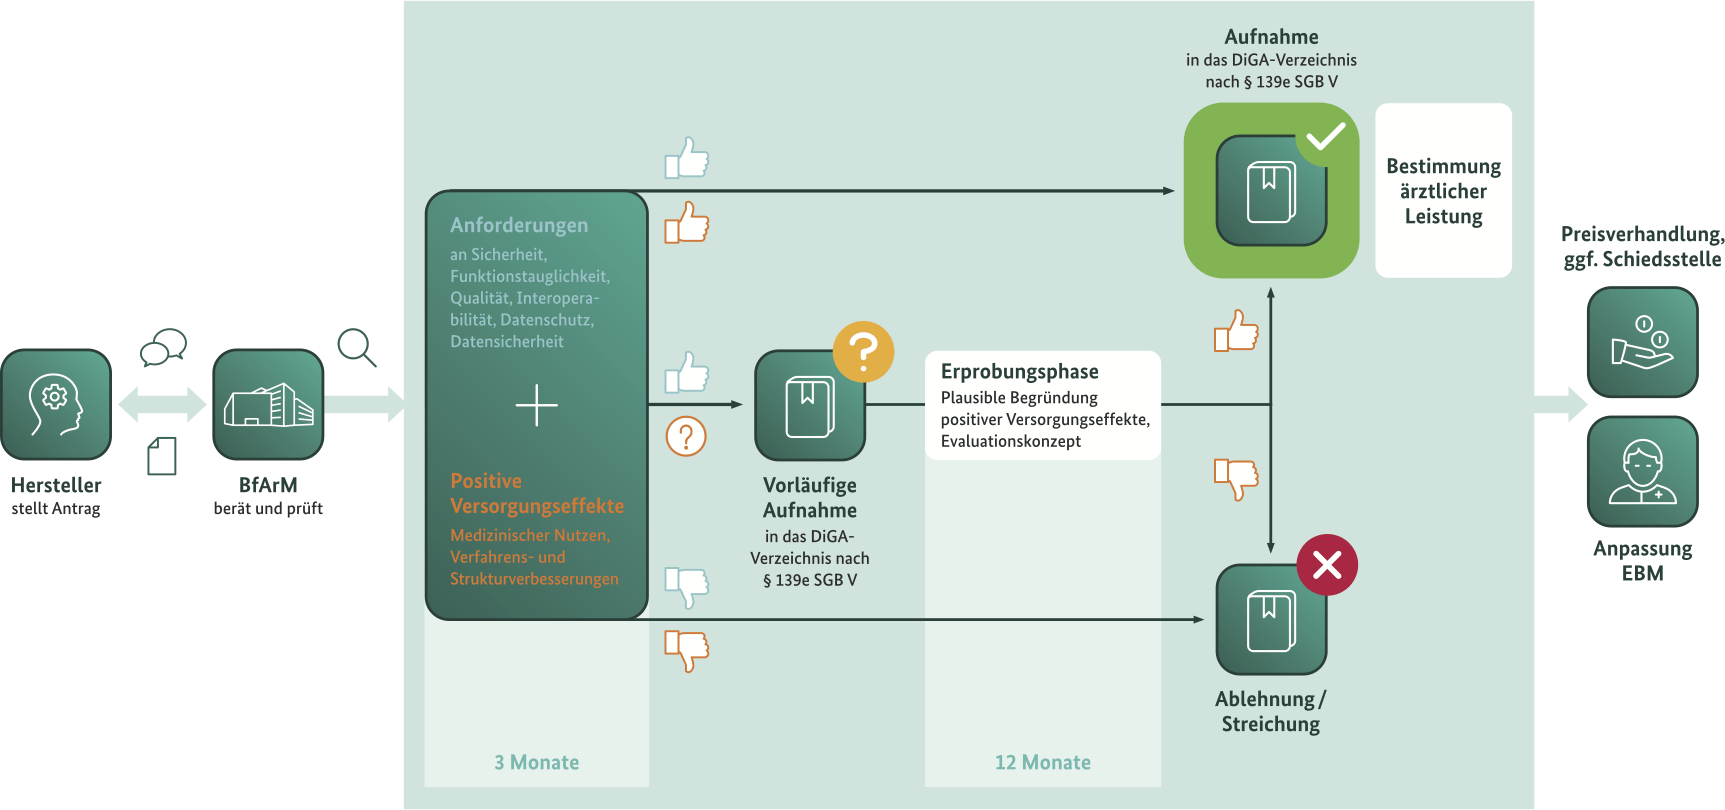
\includegraphics[width=\textwidth]{./grafiken/fast-track-verfahren}
				\caption[Ablaufdiagramm des Fast-Track-Verfahren]{Ablaufdiagramm des Fast-Track-Verfahren}
				\label{Abb-ft-Verfahren}
			\end{figure}
			In der Abbildung wird das am 27. Mai 2020 entstandene Fast-Track-Verfahren beschrieben. Im Türkisen Bereich der Abbildung sieht man, wie das Fast-Track-Verfahren abläuft. Im grünen Kasten, auf der linken Seite des Türkisen Bereichs, sieht man die 2 Voraussetzungen für eine erfolgreiche Antragsstellung die über 3 Monate hinweg vom Bundesinstitut für Arzneimittel und Medizinprodukte. Dabei gibt es die technischen Anforderungen, wie: Sicherheit, Qualität, Datenschutz etc. und die Positiven Versorgungseffekte: Medizinischer Nutzen, Verfahrens- und Strukturverbesserungen. Sollten beide Voraussetzungen erfüllt sein, wird der Antrag akzeptiert und es kommt zu Preisverhandlungen, wie man rechts oben im Türkisen Bereich sehen kann. Sollten beide Voraussetzungen nicht erfüllt sein, wird der Antrag abgelehnt, wie man rechts unten im Türkisen Bereich sehen kann. Sollten nun die technischen Anforderungen erfüllt sein, aber der Positive Versorgungseffekt noch fragwürdig sein, wird die DiGA vorläufig aufgenommen und es kommt zu einer 12-Monatigen Erprobungsphase.
		\newpage
	\section{Informationen zu den DiGAs}   
		Im folgenden Kapitel werden allgemeine Informationen, sowie Statistiken zu den DiGA wiedergegeben.
		\subsection{Fast-Track-Verfahren} 
			\begin{figure}[htbp]
				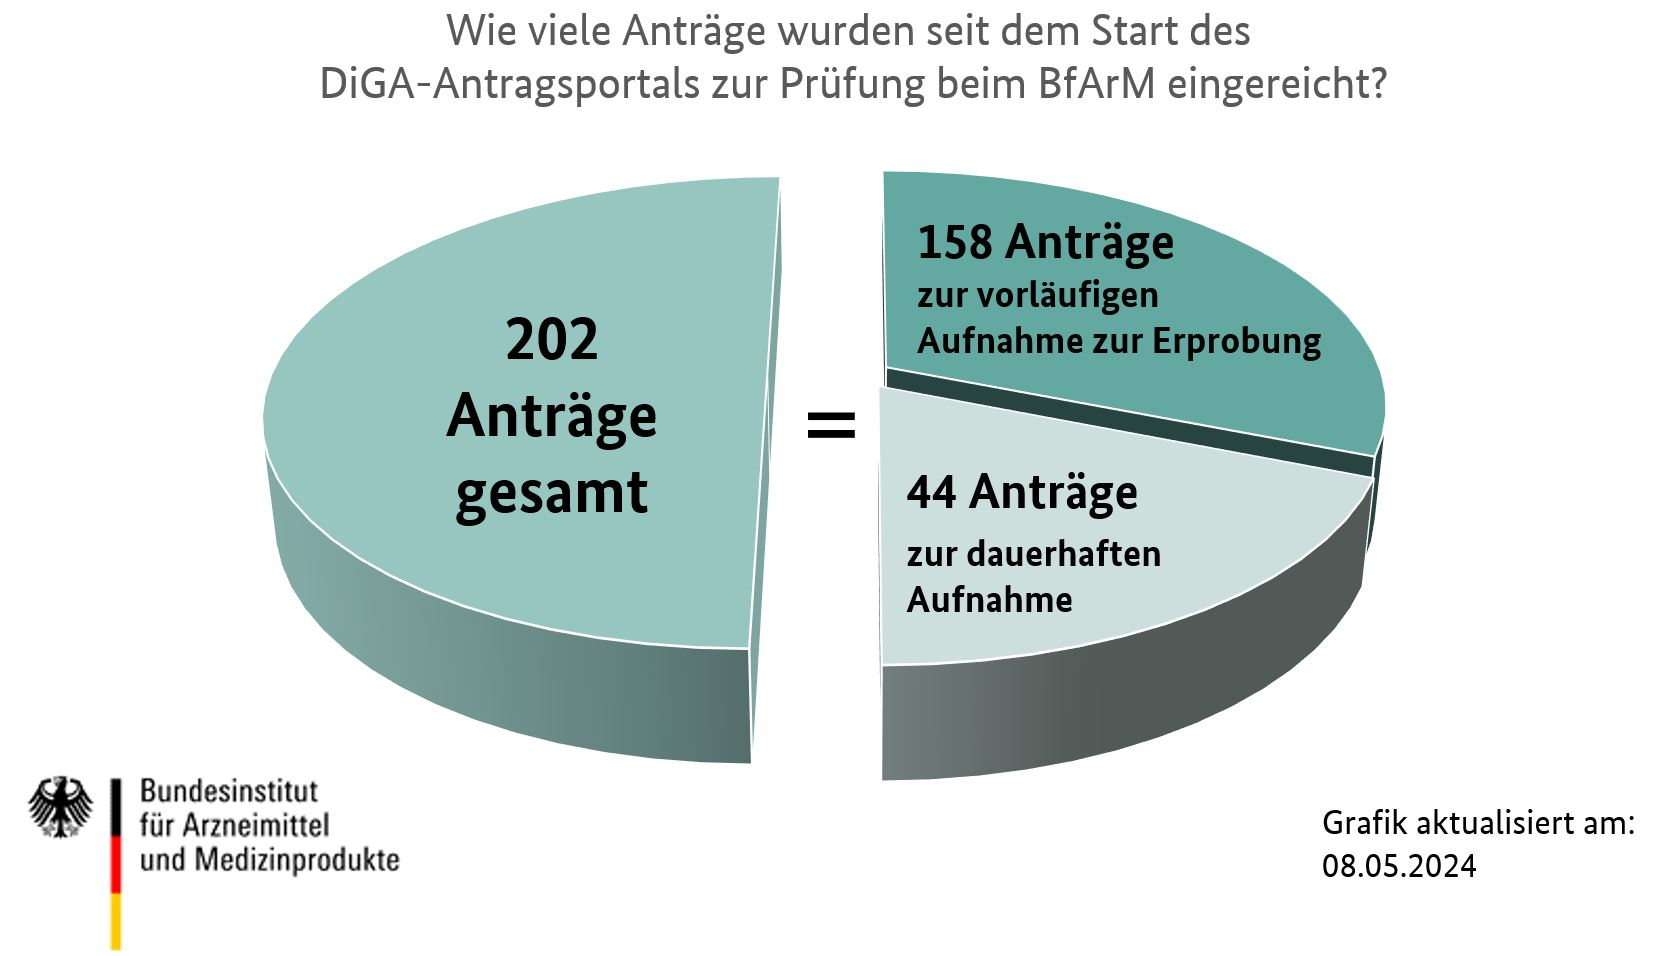
\includegraphics[width=\textwidth]{./grafiken/Anzahl_Antraege_DiGA}
				\caption[Anzahl Anträge von DiGAs]{Kuchendiagramm zur Anzahl von Anträgen von DiGAs}
				\label{Abb-antragsanzahl-diga}
			\end{figure}
			In der Abbildung kann man die Aufteilung der Gesamt Anträge sehen. Von den insgesamt 202 Anträge, wurden 44 Anträge direkt dauerhaft aufgenommen. Daraus kann man schließen das circa 75 Prozent der Anträge, zum Zeitpunkt der Antragsanstellung, noch einen ungewissen medizinischen Nutzen hatten.
			\newpage
			\begin{figure}[htbp]
				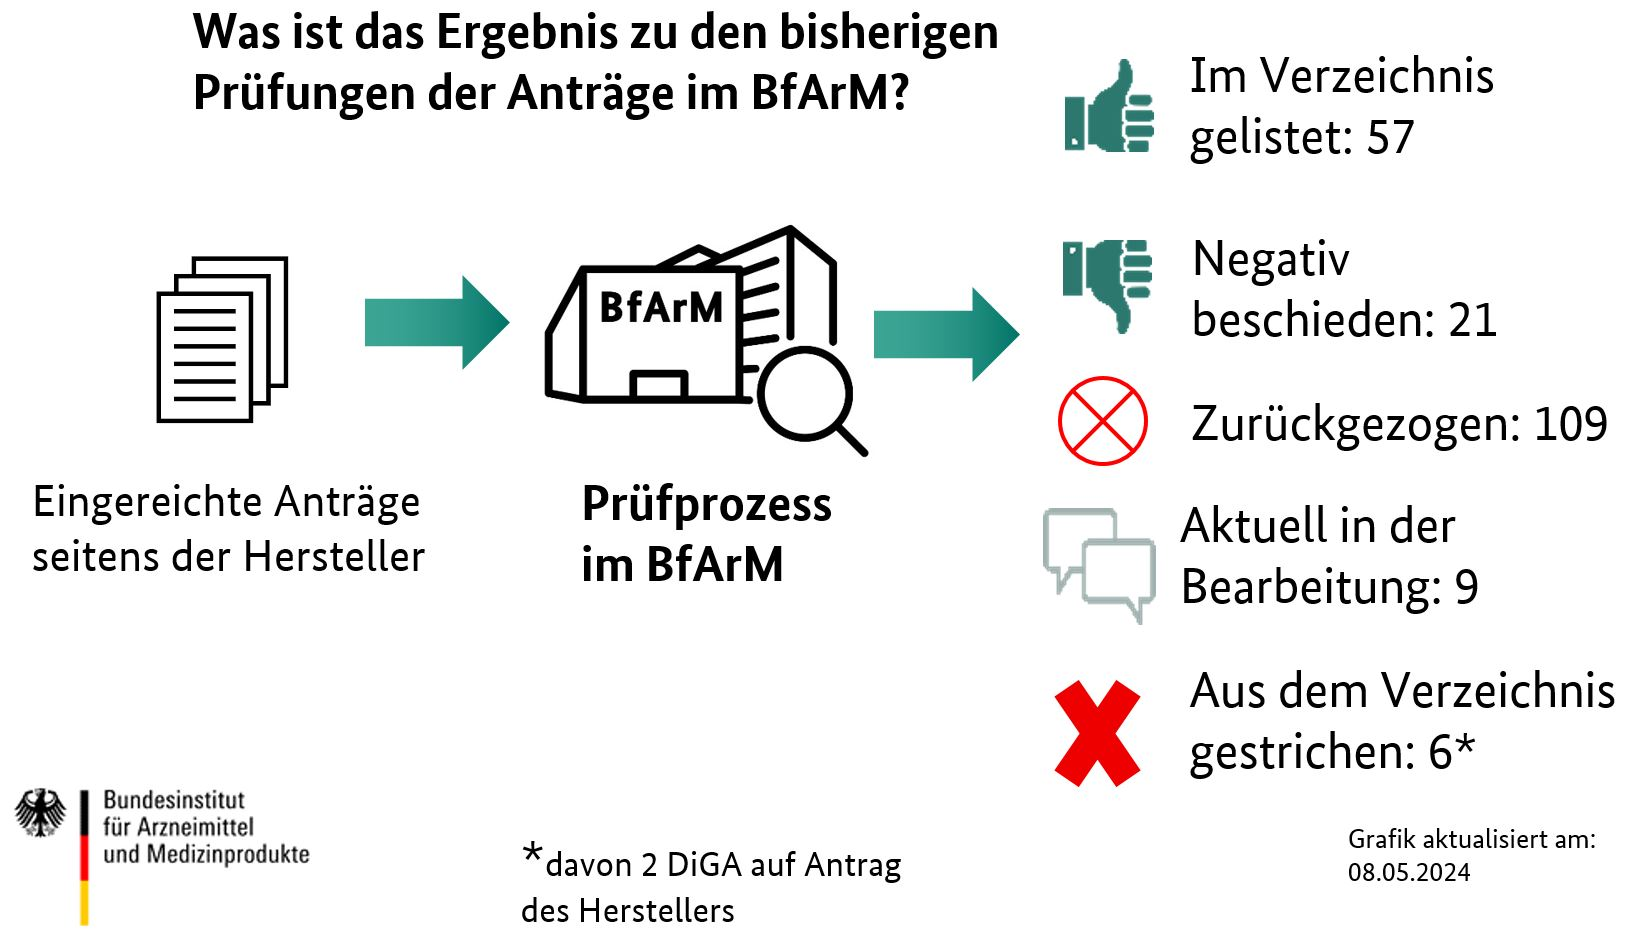
\includegraphics[width=\textwidth]{./grafiken/Ergebnis_Pruefungen_DiGA}
				\caption[Abbildung zu den Ergebnissen des Fast-Track-Verfahren]{Diagramm zu den Ergebnissen des Fast-Track-Verfahren}
				\label{Abb-ergebnisse-ft}
			\end{figure} 
			In der Abbildung kann man die Prüfergebnisse, der Anträge, des BfArM sehen. Von den 202 Anträgen wurden 109 davon zurückgezogen. Somit wurden mehr als 50 Prozent aller Anträge von den Herstellern zurückgezogen. Laut Angaben des BfArM kommt dies durch inhaltlichen Nachbesserungsbedarf bei den Anträgen zustande, denen die Hersteller nicht rechtzeitig nachkommen konnten, aufgrund der kurzen Fristen des Fast-Track-Verfahren\cite[vgl. Z. 37]{tipps-diga-antragsansteller}   
			\newpage
			\begin{figure}[htbp]
				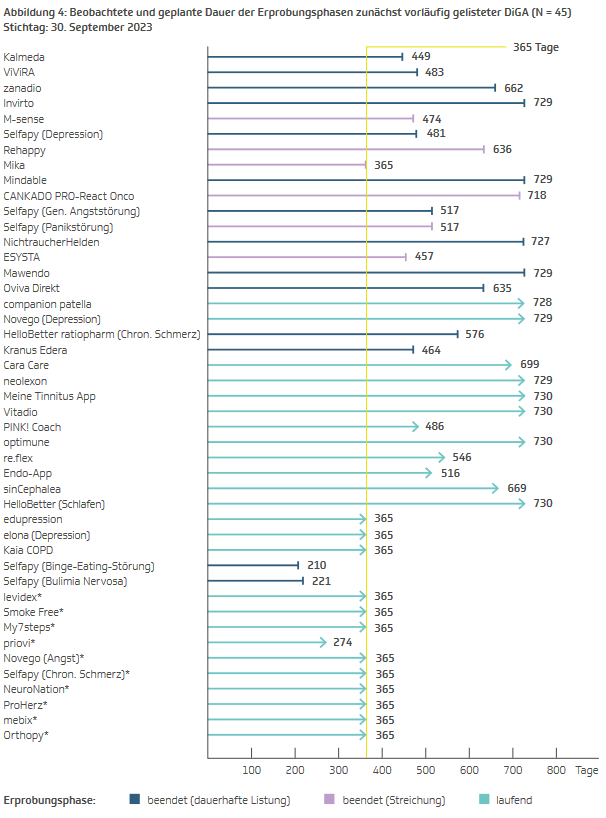
\includegraphics[height=0.5\textheight]{./grafiken/erprobungs_phase_diga}
				\centering
				\caption[Erprobungsphase von den DiGAs]{Balkendiagramm zu der Erprobungsphase der DiGAs (Stichtag: 30. September 2023)}
				\label{Abb-erprobungsphase-diga}
			\end{figure}
			In der Abbildung kann man die Beobachtete und geplante Erprobungsphase von vorläufig gelisteten DiGAs sehen. Die gelbe Linie steht im Kontext zur Abbildung, für die  Zwölfmonatige Erprobungsphase der BfArM, wie in Abbildung \ref{Abb-ft-Verfahren} zu sehen ist. Bei den DiGAs mit abgeschlossener Erprobung (30. September 2023)(blaue und pinke Linie) handelt es sich um den Zeitraum zwischen dem Listungsdatum und dem Entscheidungsdatum des BfArM, ob die DiGA dauerhaft aufgenommen oder gestrichen wird\cite[vgl. S.10]{TK-Report-2}. Von den 6 gestrichenen DiGA wurden 2 davon, auf bitte des Herstellers gestrichen wie in Abbildung \ref{Abb-ergebnisse-ft} zu sehen ist. Der Hersteller kann die Verlängerung der Erprobungsphase beantragen oder sie kann auf die Prüfphase zurückzuführen sein, die vom BfArM veranlasst wird. Um herstellerinitiierte Verlängerungen sicher zu identifizieren, wird ein Prüfzeitraum von 120 Tagen anstelle der gesetzlich vorgeschriebenen drei Monate angesetzt. Bei mehr als zwei von drei DiGA, die für die Erprobung bei Markteintritt aufgeführt sind (23 von 45), wird dieser angenommene Prüfzeitraum überschritten. Daher kann davon ausgegangen werden, dass Hersteller Verlängerungen beantragen. Es ist jedoch zu beachten, dass für zehn der 22 Anwendungen ohne bereits verlängerte Erprobungsphase zum Stichtag 30. September 2023 noch eine spätere Verlängerung möglich ist.\cite[vgl S. 10]{TK-Report-2} Wie man in der Abbildung sehen kann, ist somit die auf 1 Jahr angesetzte Erprobungsphase des BfArMs, nicht realistisch.
		\subsection{Preise und Vergütungsbeiträge der DiGAs}  
			In den ersten 12 Monaten (Erstes Listungsjahr) der DiGA, gilt ein vom Hersteller frei festgelegter Preis (sog. "tatsächlicher Preis"). Ab dem ersten Tag des 13. Monats wird der freie Herstellerpreis durch einen vom Hersteller und GKV-Spitzenverband verhandelten Vergütungsbeitrag, ersetzt. Sollte es jedoch zu keiner Einigung zwischen dem Hersteller und des GKV-Spitzenverband kommen, wird eine Schiedstelle eingeschaltet die ein Vergütungsbeitrag festlegt. Dabei ist der Vergütungsbeitrag rückwirkend, bedeutet also, sollte der Vergütungsbeitrag niedriger sein als der freie Herstellerpreis, hat die Krankenkasse einen Anspruch auf Rückzahlungen\cite[vgl. S. 11]{TK-Report-2}. Diese Preise können sich auf unterschiedliche Anwendungszeiträume beziehen, wie in Abbildung \ref{Abb-andwendungszeiträume-diga} zu sehen ist. 
			\begin{figure}[hbtp]
				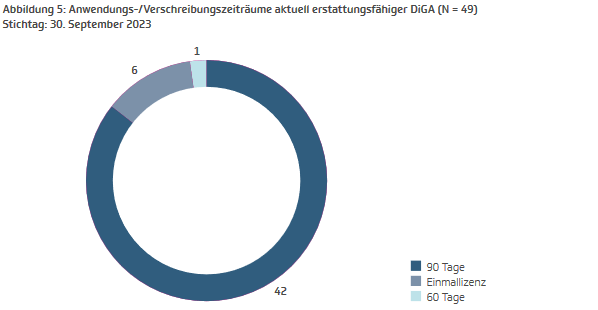
\includegraphics[width=\textwidth]{./grafiken/anwendungszeitraume_diga}
				\caption[Anwendungszeiträume von DiGAs]{Kuchendiagramm zu den Anwendungszeiträume von DiGAs (Stichtag: 30. September 2023)}
				\label{Abb-andwendungszeiträume-diga}
			\end{figure}
			Sollte es nun zum Fall kommen, das die Schiedstelle eingeschaltet werden muss, um den Vergütungsbeitrag zu bestimmen, hat diese ein Preisbemessungsmodell erstellt, die die Kosten von vergleichbaren GKV-Versorgungen im jeweiligen Anwendungsgebiet untersucht. Als Beispiel war es bislang in allen Verfahren für digitale Gesundheitsanwendungen im Bereich psychischer Erkrankungen üblich, eine persönliche Gruppentherapie mit kognitiver Verhaltenstherapie als festen "Preisanker" anzunehmen. Diese Methodik wird auch in den anderen Bereichen angewendet. Die genaue Kostenberechnung für die vergleichbare Versorgung erfolgt für den Zeitraum, in dem die entsprechende DiGA genutzt wird.\cite[vgl. S. 13]{TK-Report-2} Also in der Regel 90 Tage (1 Quartal), wie in Abbildung \ref{Abb-andwendungszeiträume-diga} zu sehen ist. Basierend auf den geschätzten Kosten des Referenzpreises wird eine "Nutzenanpassung" in Form eines prozentualen Aufschlags vorgenommen. Dieser richtet sich hauptsächlich nach einer Bewertung des Ausmaßes des positiven Versorgungseffekts (gering/mittel/hoch) und der Qualität der Studien (gering/mittel/hoch), die von der Schiedsstelle vorgenommen wird. Zusätzlich zu den geschätzten Kosten des Preisankers werden auch, in Einzelfällen, andere qualitative Faktoren berücksichtigt, wie beispielsweise die Epidemiologie der Erkrankung, alternative Therapiemöglichkeiten usw. Dabei werden auch Selbstzahler- und europäische Vergleichspreise der digitalen Gesundheitsanwendungen mit einer Gewichtung von bis zu 15 Prozent einbezogen.\cite[vgl. S. 13]{TK-Report-2} Wie in Abbildung \ref{Tab-preise-diga} zu sehen ist, gibt es keine großen Unterschiede zwischen den Vergütungsbeiträge, die von der Schiedstelle festgelegt oder den Herstellern und GKV-Spitzenverband vereinbart wurden. 
			\begin{figure}[htbp]
				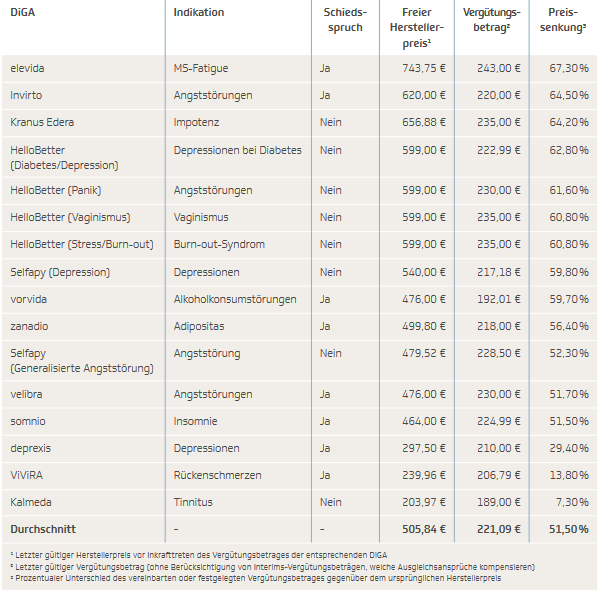
\includegraphics[width=\textwidth]{./grafiken/tabelle_preise_diga}
				\caption[Gegenüberstellung der freien Herstellerpreise und verinbarten oder festgelegten Vergütungsbeiträge]{Tabelle zur Gegenüberstellung der freien Herstellerpreise und vereinbarten oder festgelegten Vergütungsbeiträge (Stichtag: 30. September 2023)}
				\label{Tab-preise-diga}
			\end{figure}
		\subsection{Anwendungsgebiete}
			\begin{figure}[htbp]
				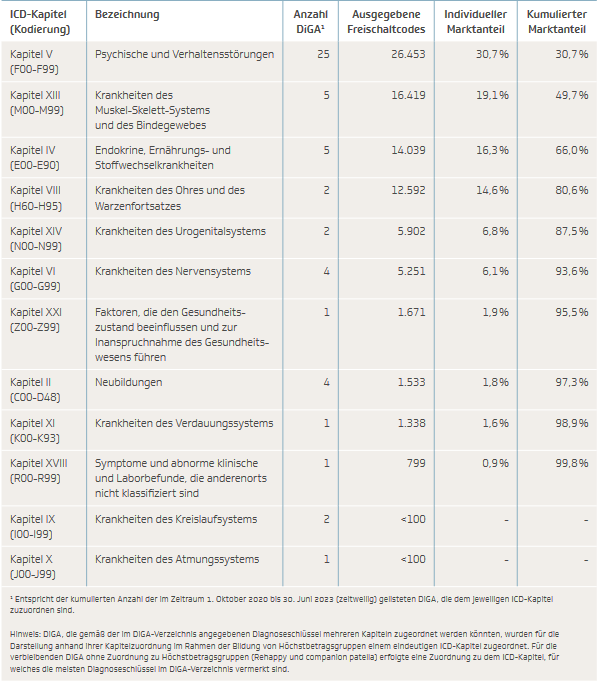
\includegraphics[height=0.5\textheight]{./grafiken/tabelle_anwendungsfelder_diga}
				\caption[Anwendungsfelder der DiGA]{Tabelle zu den Anwendungsfelder (Zeitraum: 1. Oktober 2020 - 30. Juni 2023)}
				\label{Tab-anwendungsfelder-diga}
			\end{figure}
			In der Tabelle, kann man sowohl die verteilten Freischaltcodes, als auch die Marktanteile der jeweiligen Anwendungsfelder sehen. Es wurden im angegeben Zeitraum insgesamt 86.213 Freischaltcodes ausgegeben. In der Tabelle, kann man deutlich sehen das mit circa 50 Prozent der DiGAs im Anwendungsfeld der Psychischen und Verhaltensstörungen sind. Diese sind mit einem Individuellem Marktanteil von 30,7 Prozent auch die häufigsten verordneten DiGAs.
			\newpage
			\begin{figure}[htbp]
				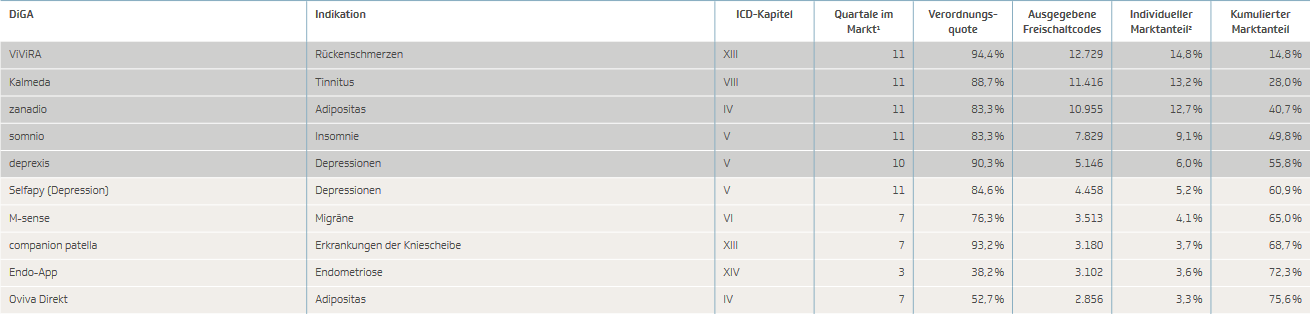
\includegraphics[width=\textwidth]{./grafiken/tab_diga_verteilung}
				\caption[Freigegebene Freischaltcode je DiGA]{Tabelle zu Freigegebenen Freischaltcodes je DiGA (Zeitraum: 1. Oktober 2020 - 30. Juni 2023)}
				\label{Tab-freischaltcodes-je-diga}
			\end{figure}
			In der Tabelle kann man die Top 10 verteilten DiGAs im DiGA-Verzeichnis sehen. Diese 10 machen 75,6 Prozent aller ausgegeben Freischaltcodes aus. In der Tabelle wird nochmals der Marktanteil von 30,7 Prozent im Anwendungsfeld der Psychischen- und Verhaltensstörungen bestätigt mit somnio, deprexis und Selfapy (Depressionen).  
	\section{Informationen zu den Nutzern und Verordneten}
		Im folgenden Kapitel werden allgemeine Information, sowie Statistiken zu den Nutzern und Verordneten der DiGAs wiedergegeben.
		\subsection{Nutzer}
			
				 
\bibliographystyle{abbrv}
\bibliography{seminar_arbeit_marcelo}
\end{document}